\section{Metodologia}
\label{sec:metodologia}

Spiegare notazione grafo, parametri, usiamo 1 simbolo per indicare gli score. Quando scriviamo una sezione qui sotto 2.x, se ci serve della notazione poi andiamo a metterla qui. 
Fare dei paragrafi per BM25, PageRank, Hits, LSA, ES.

%In questo paragrafo, si illustreranno i metodi sviluppati e sperimentati con le
%attivit\`a di laboratorio. Le notazioni e tutti gli aspetti non banali dovranno
%essere spiegati. Naturalmente, la notazione di un paragrafo non dovr\`a essere
%reintrodotta nei paragrafi successivi, di conseguenza, la notazione non dovr\`a
%essere ambigua.

\subsection{Approccio}
\label{sec:approccio}

%Vogliamo max la map. Usando treceval spiegare cos'e'. Spiegare brevemente il lavoro, molto veloce dire che abbiamo lavorato insieme dopo la prima sessione in lab. Usato python, con \texttt{numpy} per matrici, matplotlib per plottare, networkx per grafi, git per versionamento, latex per i report.
%Il nostro scopo e' ottenere un valore di map il piu' elevato possibile. Per calcolarla e verificarne il cambiamento durante le varie versione del codice utilizziamo \texttt{treceval}, esso e' il tool standard usato dalla "TREC community" per valutare un'esecuzione ad hoc, dandole il file contenete i risultati e un set standard di risultati giudicati.  

%Abbiamo deciso di utilizzare un approccio probabilistico poiche' fornisce una formalizzazione piu' pulita di cosa volgiamo che faccia un sistema IR: dare documenti rilevanti agli utenti. 
%Inoltre per via delle nostre conoscenze abbiamo voluto utilizzare il linguaggio Python per dare corpo ai progetti. Inoltre vi sono diverse librerie che implementano molti metodi utili per tale corso e per garantire buone performance al codice: \texttt{numpy} usata per la gestione delle matrici, \texttt{matplotlib} utilizza per effettuare i plot (grafici) dei risultati ottenuti, \texttt{networkx} utilizzata per la creazione e gestione dei grafi.
%Oltre a \texttt{Python} abbiamo utilizzato altri software per il lavoro. E' stato usato \texttt{Git}, e' un sistema di versionamento distribuito, per lo scambio del codice e l'aggiornamente delle diverse versioni di quest'ultimo. Infini \texttt{latex} per la scrittura dei pdf di report.
%Per ogni esercitazioni è stato utilizzato un approccio di gruppo. Dopo la prima sessione di laboratorio di ogni esercitazione ci siamo ritrovati per la scrittura del codice, la discussione sui risultati e la stesione del report.

\subsection{Indicizzazione} \label{sec:metodi-di-indic}

Qui va il contenuto del laboratorio n. 2.

\subsection{Reperimento}
\label{sec:metodi-di-reper}

Qui va il contenuto del laboratorio n. 3. Esso rappresenta la \textit{baseline}.

\subsection{Relevance Feedback}
\label{sec:relevance-feedback}

Qui va il contenuto del laboratorio n. 4.

\subsection{PageRank}
\label{sec:pagerank}

Qui va il contenuto del laboratorio n. 5.

\subsection{Latent Semantic Analysis}
\label{sec:lsa}

Qui va il contenuto del laboratorio n. 6.

\subsection{Hyper-linked Induced Topic Search}
\label{sec:hits}

Qui va il contenuto del laboratorio n. 7.

\subsection{Evolution Strategy}
\label{sec:es}

Per ottimizzare gli algoritmi di reperimento abbiamo scelto di utilizzare un Evolution Strategy~\cite{back1996evolutionary} (ES) che e' una tecnica di ottimizzazione basata sui principi che regolano l'evoluzione. Tecniche di questo tipo sono piu' robuste rispetto ai metodi di ricerca lineare per quanto riguardo i massimi locali. Il loro svantaggio consiste nel maggior numero di valutazioni richieste. Nel nostro contesto una valutazione impiega circa 3-15 secondi a seconda della complessita' del metodo di reperimento. Cio' permette di eseguire l'algoritmo di ottimizzazione in un tempo accettabile.

I parametri che abbiamo scelto di ottimizzare cambiano in base alla funzione di reperimento (e quindi del laboratorio). Per il laboratorio 3, 4, 6 abbiamo scelto di ottimizzare $k_1, b$. Ignoriamo $k_2$ in quando abbiamo visto che non ci sono termini ripetuti nelle query e quindi tale termine non influisce sul punteggio. Per il laboratorio 5 ottimizziamo $k_1, b, \alpha$. Per il laboratorio 7 ottimizziamo $k_1, b, \alpha, \beta, \gamma$. Per lo pseudo relevance feedback del laboratorio 4 il numero di documenti considerati rilevanti $R = 50$, mentre per l'\textsc{lsa} del laboratorio 6 il numero di documenti da riordinare $N = 30$, e il numero di dimensioni per la riduzione $m=2$ (tali parametri sono interi e non si prestano ad un ottimizzazione tramite ES). La funzione da massimizzare e' la Mean Average Precision.

Figura \ref{fig:es_all} riporta l'andamento della MAP durante l'ottimizzazione della funzione di reperimento dei laboratori. 
\begin{figure*}
        \centering
        \begin{subfigure}[htpb]{0.475\textwidth}
            \centering
            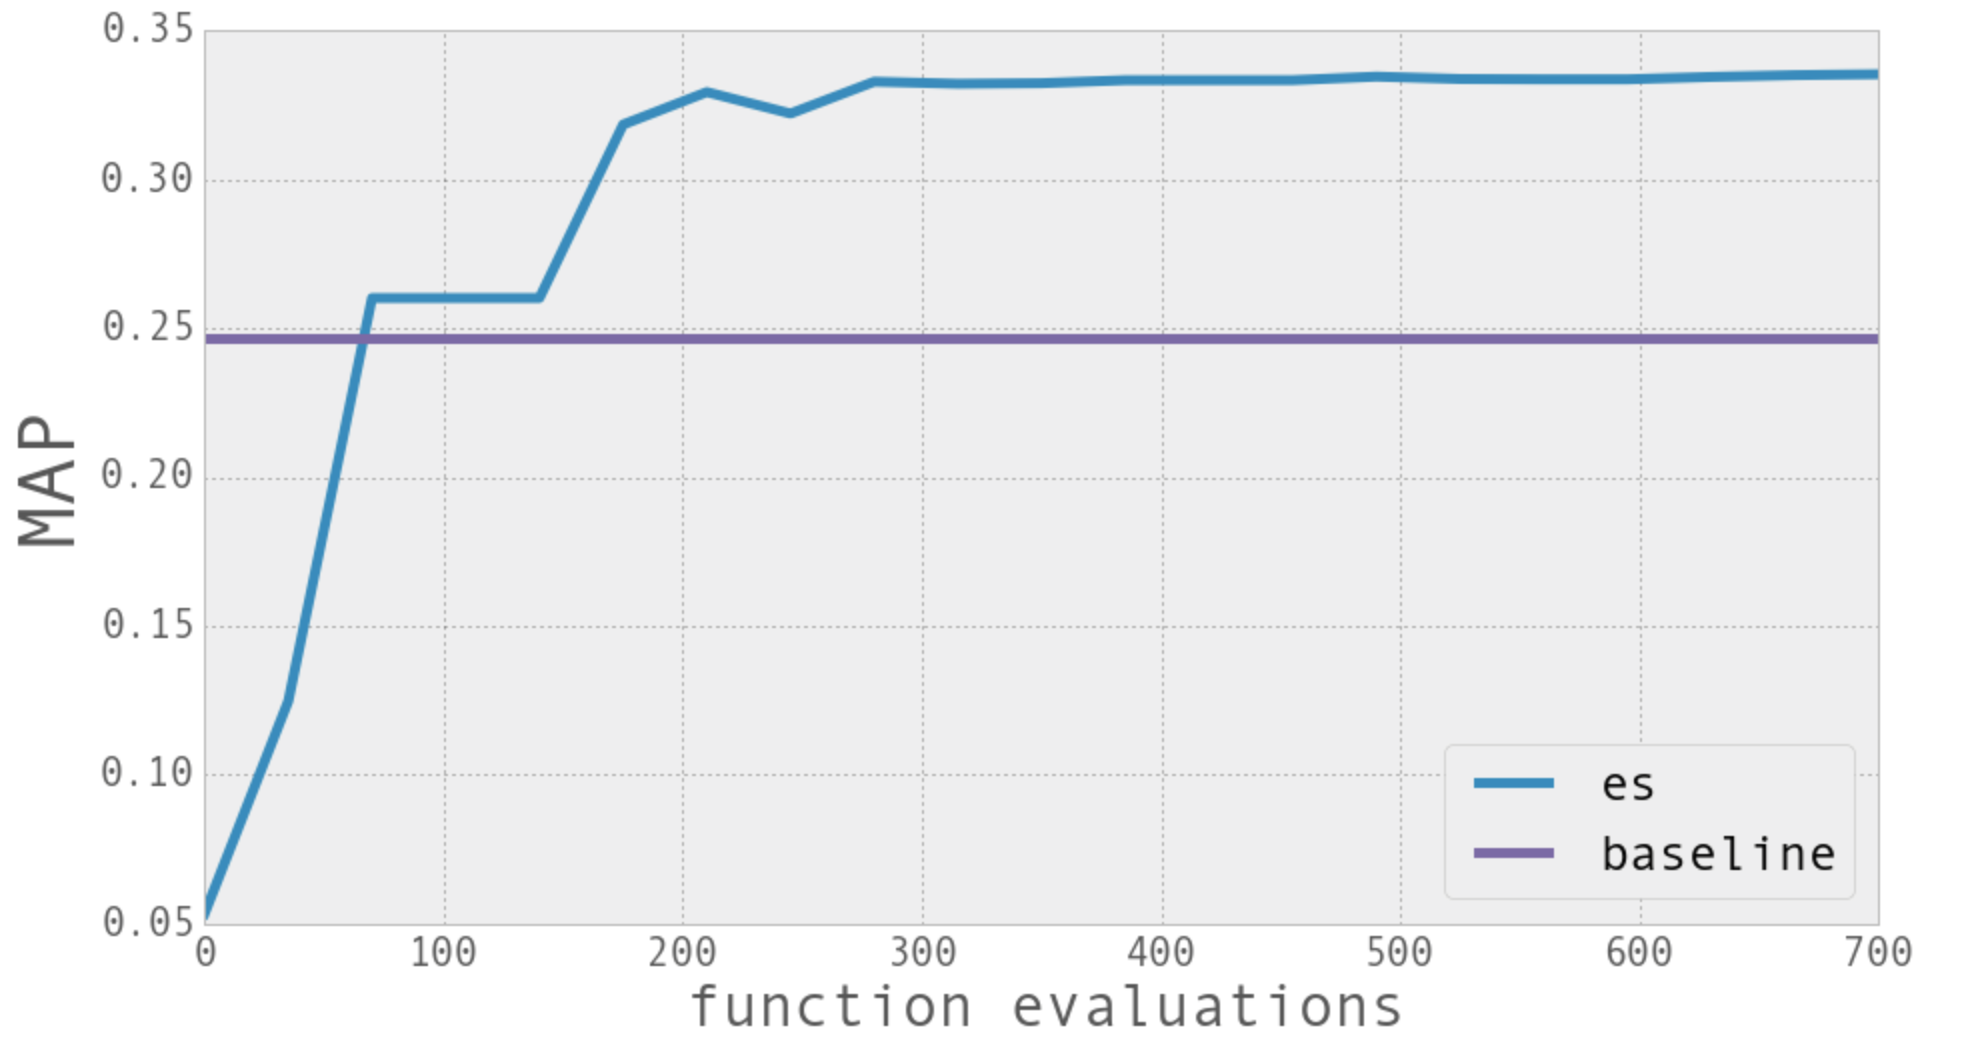
\includegraphics[width=\textwidth]{figures/es_lab3.png}
            \caption[Network2]%
            {{\small Laboratorio 3 (\textsc{baseline})}}    
            \label{fig:es_lab3}
        \end{subfigure}
        \hfill
        \begin{subfigure}[htpb]{0.475\textwidth}  
            \centering 
            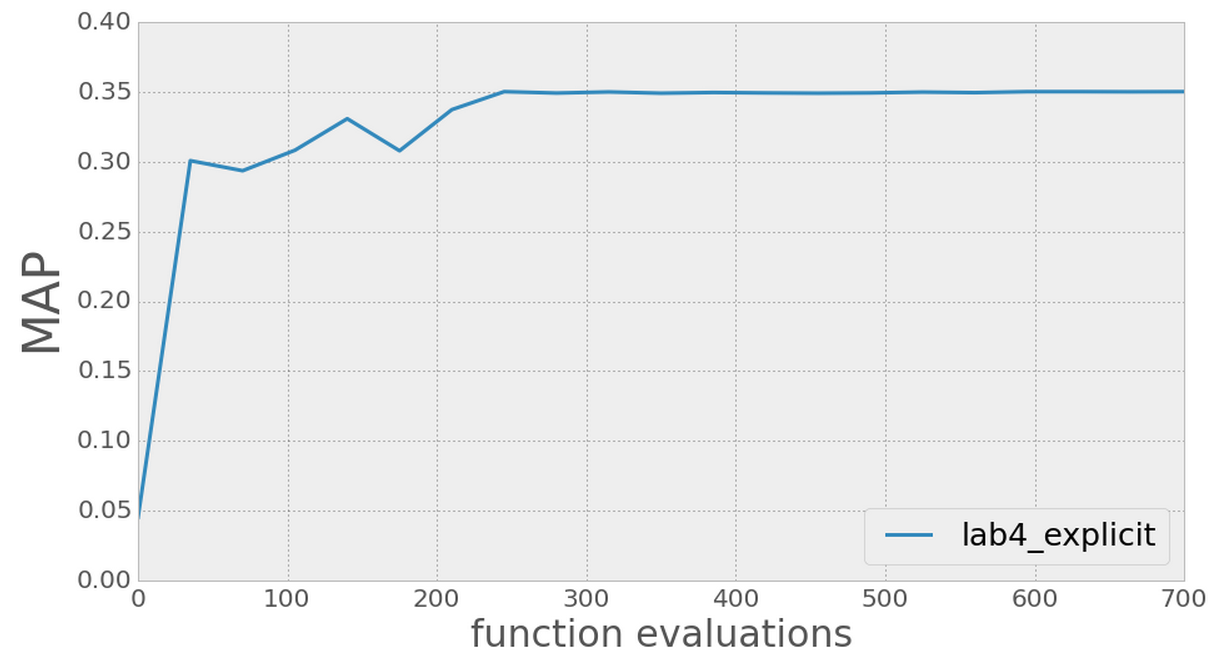
\includegraphics[width=\textwidth]{figures/es_lab4_e.png}
            \caption[]%
            {{\small Laboratorio 4 (\textsc{RF} esplicito)}}    
            \label{fig:es_lab4_esp}
        \end{subfigure}
        \vskip\baselineskip
        \begin{subfigure}[htpb]{0.475\textwidth}   
            \centering 
            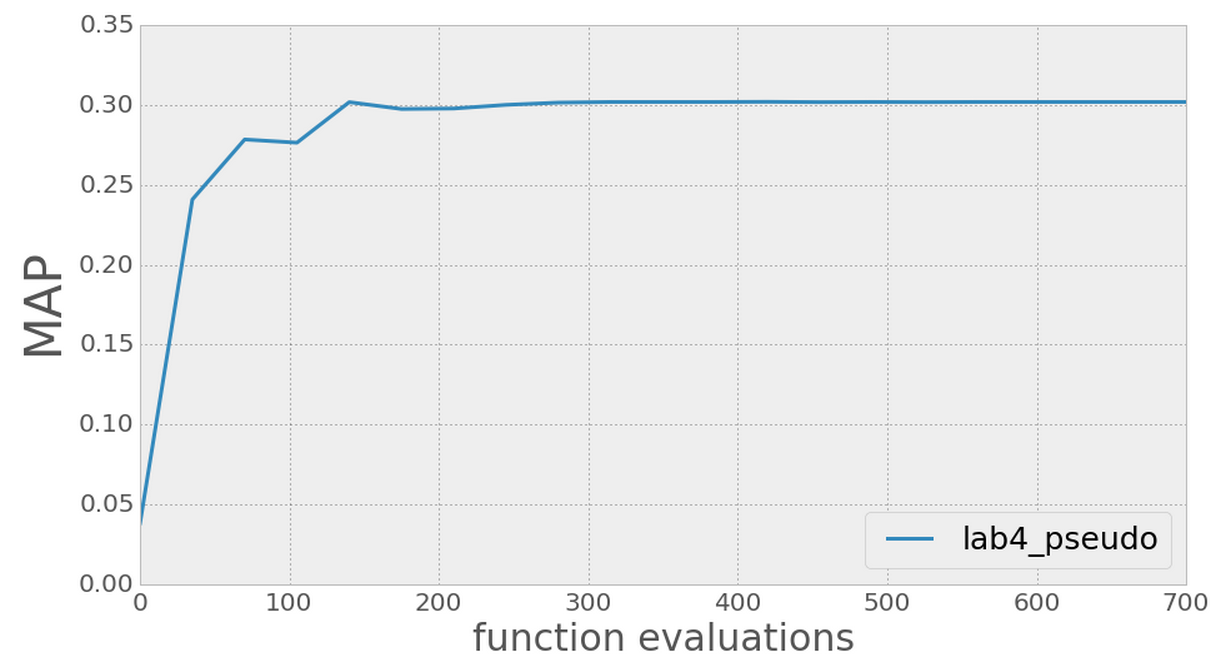
\includegraphics[width=\textwidth]{figures/es_lab4_p.png}
            \caption[]%
            {{\small Laboratorio 4 (\textsc{RF} pseudo)}}    
            \label{fig:es_lab4_pse}
        \end{subfigure}
        \quad
        \begin{subfigure}[htpb]{0.475\textwidth}   
            \centering 
            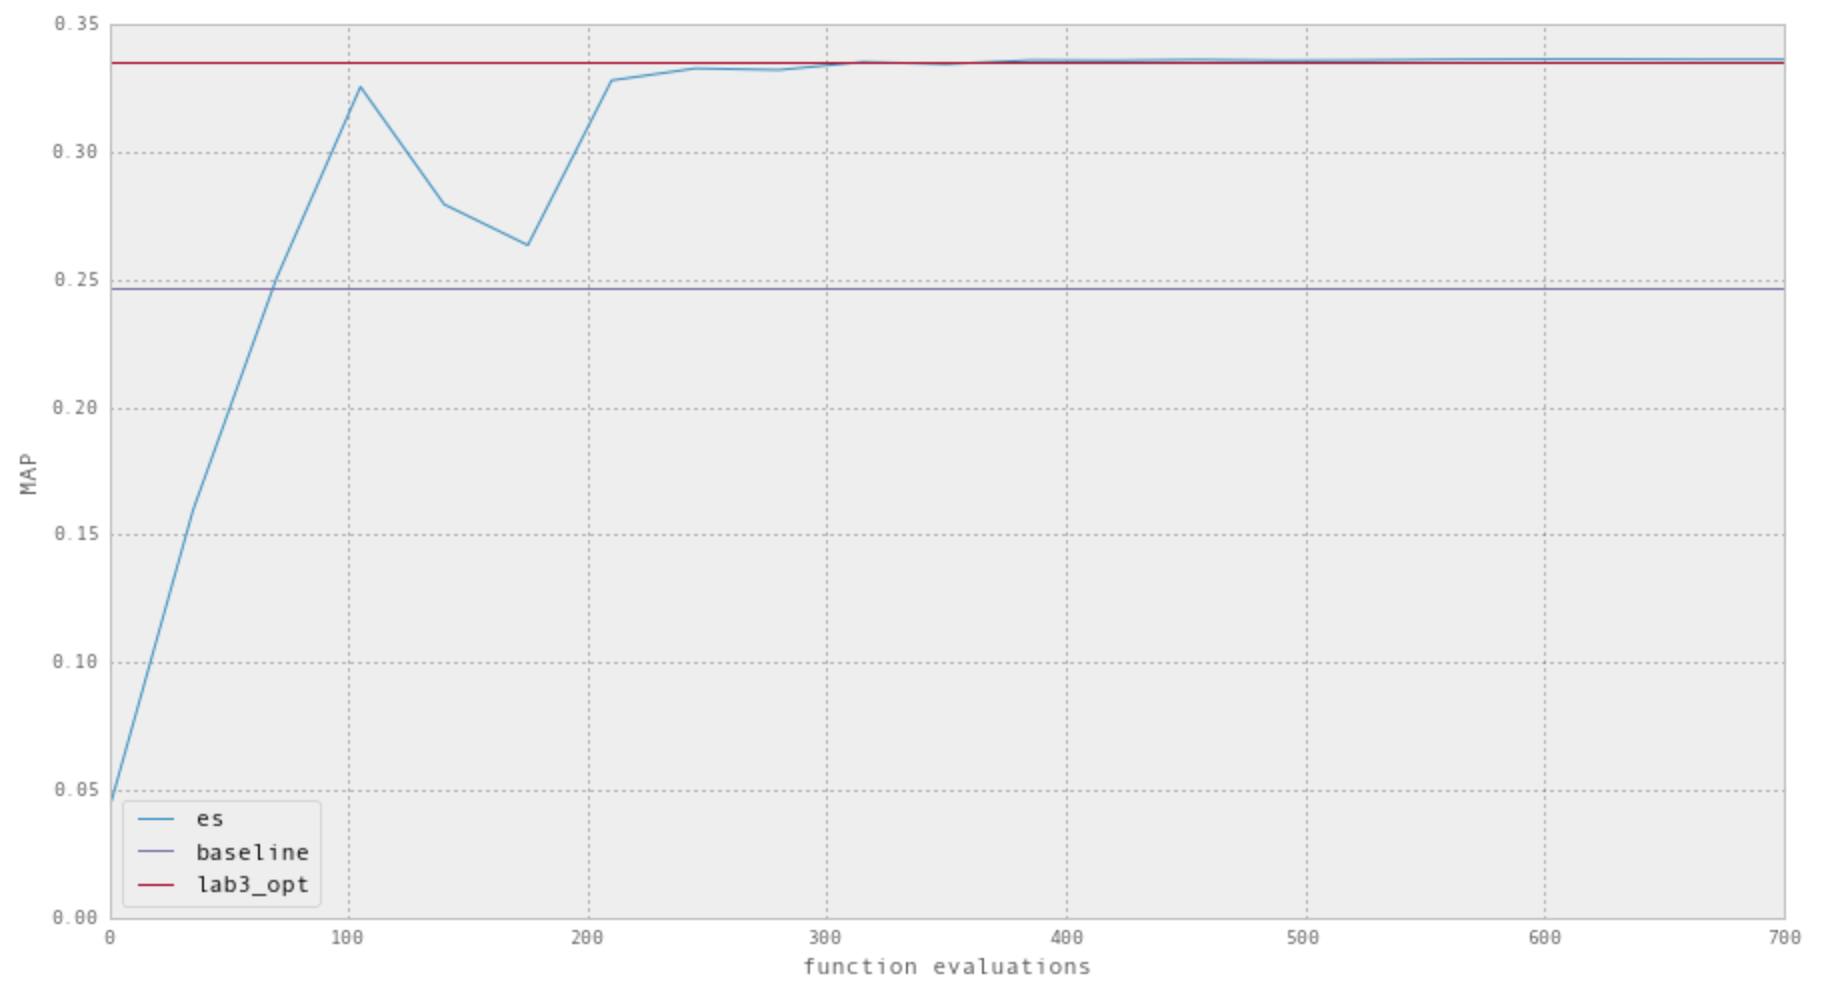
\includegraphics[width=\textwidth]{figures/es_lab5.png}
            \caption[]%
            {{\small Laboratorio 5 (\textsc{pagerank})}}    
            \label{fig:es_lab5_esp}
        \end{subfigure}
        \vskip\baselineskip
        \begin{subfigure}[htpb]{0.475\textwidth}  
            \centering 
            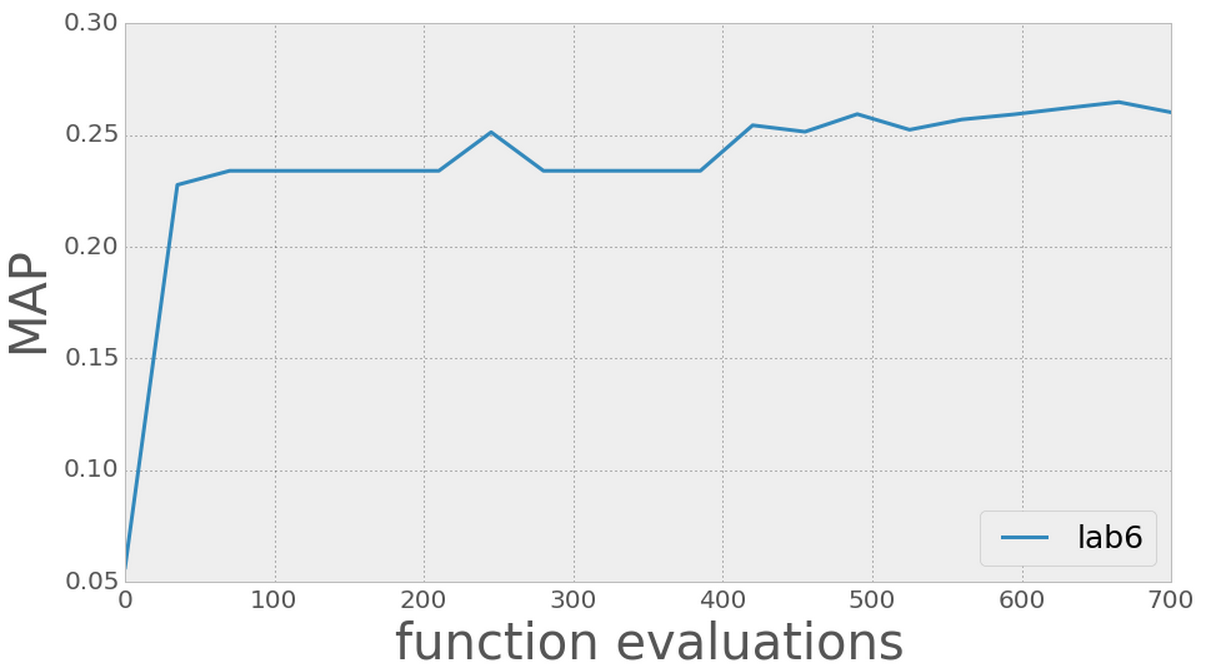
\includegraphics[width=\textwidth]{figures/es_lab6.png}
            \caption[]%
            {{\small Laboratorio 6 (\textsc{lsa})}}    
            \label{fig:es_lab6}
        \end{subfigure}
        \quad
        \begin{subfigure}[htpb]{0.475\textwidth}   
            \centering 
            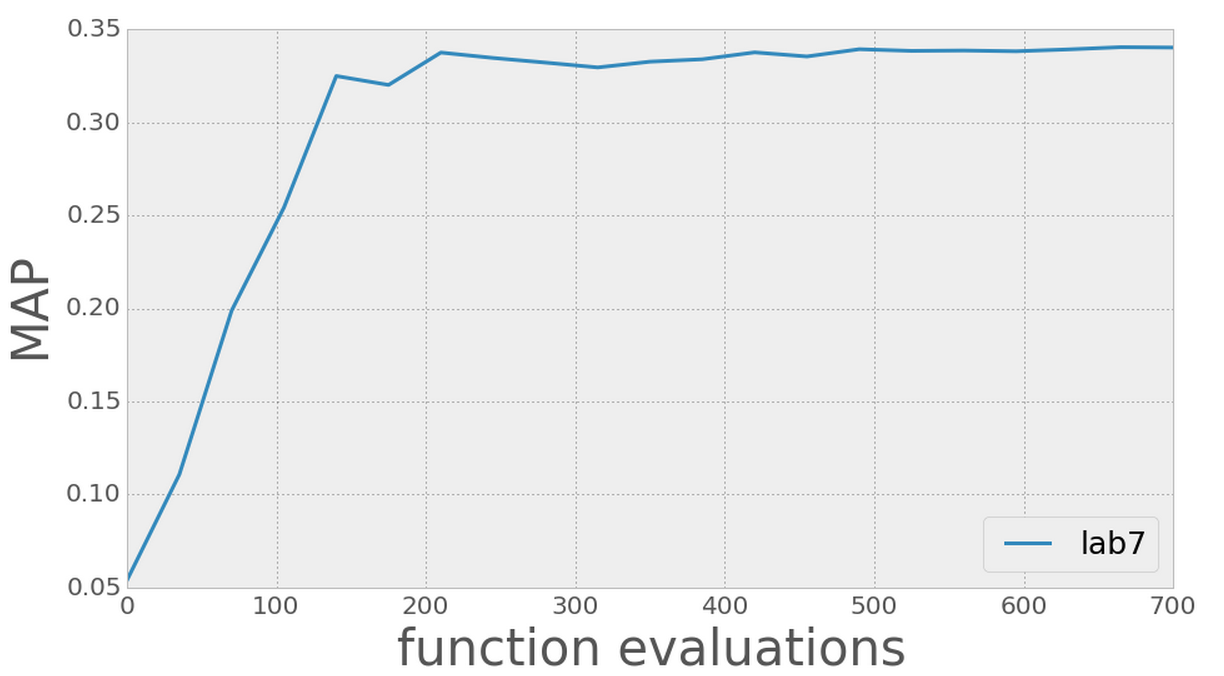
\includegraphics[width=\textwidth]{figures/es_lab7.png}
            \caption[]%
            {{\small Laboratorio 7 (\textsc{hits})}}    
            \label{fig:es_lab7}
        \end{subfigure}
        \caption[ The average and standard deviation of critical parameters ]
        {\small Valore MAP durante iterazioni dell'ES, per le funzioni di reperimento dei vari laboratori.} 
        \label{fig:es_all}
\end{figure*}
Tabella \ref{tab:es} riporta i risultati dell'ottimizzazione.
\begin{table}[htpb]

\begin{center}
\begin{tabular}{|c|c|c|}
\hline
metodo & parametri ottimizzati & MAP \\
 \hline
\textsc{baseline} & $k_1 = 0.0253, b = 0.0221$ & $0.3354$ \\
\textsc{rf} esplicito & $k_1 = 0.02065, b = 0.0$ & $0.3504$ \\
\textsc{rf} pseudo & $k_1 = 0.02065, b = 0.0$ & $0.3022$ \\
\textsc{pagerank} & $k_1 = 0.0237, b = 0.0, \alpha=0.7832$ & $0.3366$ \\
\textsc{lsa} & $k_1 = 0.0087, b = 0.0$ & $0.2648$ \\
\textsc{hits} & $k_1 = 0.0247, b = 0.0185, \alpha=1.0, \beta=0.1098, \gamma=0.0549$ & $0.3405$ \\
\hline
\end{tabular}
\end{center}
\caption{Risultati ottimizzazione con ES per le funzioni di reperimento dei vari laboratori.}
\label{tab:es}
\end{table}

Grazie all'ES si e' ottenuto un notevole miglioramento rispetto alla prima versione dove i parametri sono stati scelti empiricamente, e la MAP si aggirava attorno al $0.25$. Inoltre dai grafici si puo' notare come l'algoritmo di ottimizzazione sia molto robusto, dato che dopo $\sim{300}$ valutazioni e' gia' molto vicino alla configurazione ottima. I risultati dell'ottimizzazione vengono discussi in Sezione \ref{sec:risult-sper}.

\subsection{Altri metodi}
tipo lucene
\label{sec:altri-metodi}

Se sono stati sviluppati altri metodi, descriverli qui.

